\section{Control and Status Register Files}
Hardware designs often have to be configured from outside of the hardware in order to be used properly. These settings need to be stored in the hardware. Furthermore, they also need to be accessible to read out the current configuration along with additional status information.\\
For this purpose registers are used, which are called Control and Status Registers (CSR). They are typically accessed via a host interface by the software and are directly connected to the logic of the hardware design (fig.~\ref{fig::csr}). Additionally a register can be split into multiple fields, wich can be accessed by the hardware separately. In contrast, the software is only able to read or write an entire register.
\begin{figure}[h]
 \centering
 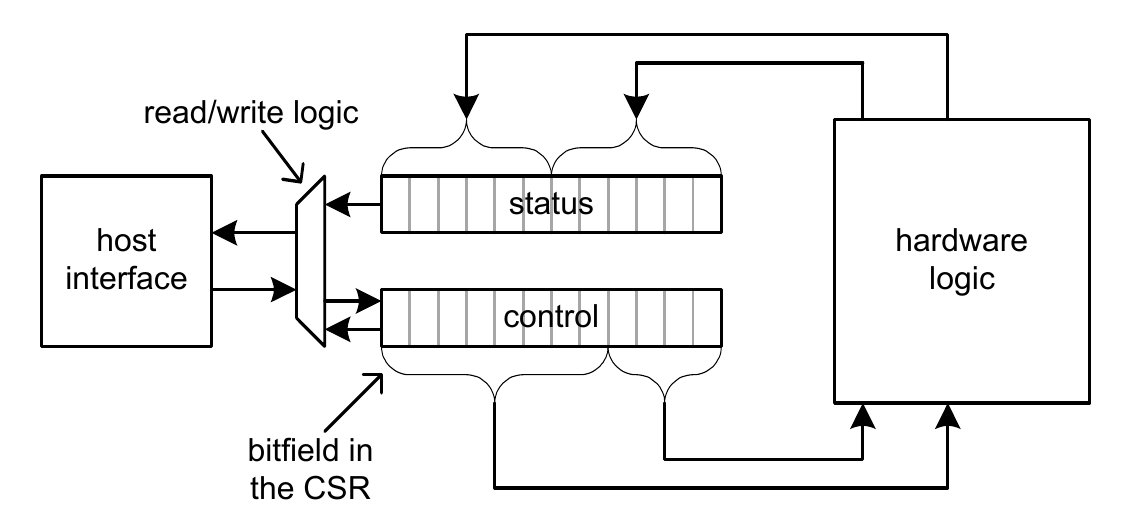
\includegraphics[width=252pt]{images/csr.png}
 \caption{Control and Status Register \cite{leber_diss}}
\label{fig::csr}
\end{figure}

In general register files (RFs) consist of multiple CSRs. They appear as a linear address space (fig.~\ref{fig::rf}) and are often mapped into the address space of the host system. This simplifies the read and write accesses by the software.
\begin{figure}[h]
 \centering
 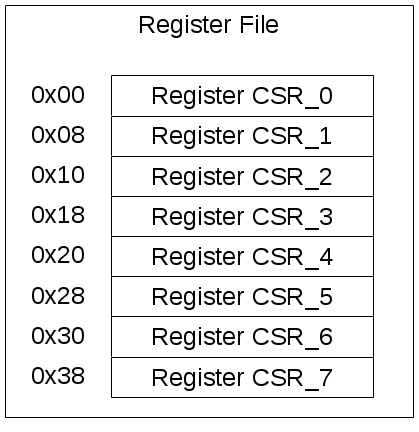
\includegraphics[width=130pt]{images/rf.png}
 \caption{Address Map of a Register File}
\label{fig::rf}
\end{figure}
